\documentclass[10pt]{beamer}
% TODO: nested NFT
% TODO: 2022/878 zk-creds: Flexible Anonymous Credentials from zkSNARKs and Existing Identity Infrastructure (Ian Miers) https://twitter.com/secparam/status/1580336115114209280
% TODO: Uniswap Permit2

\usetheme[progressbar=frametitle,numbering=none]{metropolis}
\usepackage{appendixnumberbeamer}

\usepackage{booktabs}

\usepackage{pgfplots}
\usepgfplotslibrary{dateplot}
\usetikzlibrary{positioning,arrows.meta}
\usepackage[absolute,overlay]{textpos} % for textblock* env

\usepackage{siunitx}\sisetup{group-separator={,}}
\usepackage[normalem]{ulem}
\usepackage{fontawesome5}
\usepackage{hyperref}
\newcommand{\github}[1]{%
   \href{#1}{\faGithubSquare}%
}

\usepackage{xspace}
\newcommand{\themename}{\textbf{\textsc{metropolis}}\xspace}

\title{Ethereum token standard catalog}
\subtitle{in-house seminar}
\date{2025-09-09}
\author{Jeongho Jeon}
\institute{DSRV}
\titlegraphic{\hfill\includegraphics[height=3.0ex]{dsrv_logo_master_black}}

\begin{document}

\begin{textblock*}{3cm}(0.95\paperwidth,0.97\paperheight)
{\fontsize{2pt}{2.4pt}\selectfont\color{gray}version 20250909}
\end{textblock*}

\maketitle

\begin{frame}[fragile]{Quick Reference}

\begin{itemize}
  \item Ethereum token
  \item ERC-20
  \item receive function
  \item refund (escrew)
  \item gasless with Permit
  \begin{itemize}
    \item ERC-2612 (ERC20Permit)
    \item ERC-3009 Authorization
  \end{itemize}
  \item memo
  \item ERC-3643 Permissioned Token
  \item ERC-7291 PBM
  \item ERC-4626 Vault
  \item rebase token
  \item Fireblocks ERC20F
  \item privacy
  \item ZKPassport
  \item token checklist
\end{itemize}

\end{frame}

\begin{frame}[fragile]{Ethereum token}
\begin{itemize}
  \item native token \textbf{ETH} vs smart contract token \textbf{ERC-20}
  \item \textbf{WETH} (wrapped ETH) makes ETH usable like an ERC-20.
  \item Protocols (e.g. Uniswap) auto-wrap ETH for simpler implementation.
  \item ERC-7528 defines ETH's virtual token address as \texttt{0xeeee\ldots ee}.
\end{itemize}

Token Model
\begin{itemize}
  \item Each token smart contract keeps a balance sheet in its own state (storage).
  \item To know an account's holdings, you must query all token contracts.
  \item Some chains like Aptos, Sui, and NEAR store all token information under the account.
\end{itemize}
\end{frame}

\begin{frame}[fragile]{Ethereum token}
Token Storage
\begin{itemize}
  \item Token contracts store a \texttt{account \textrightarrow\  balance} mapping.
  \item Because accounts are hashed (see ``Layout of State Variables in Storage''), you cannot read a balance table from contract storage directly.
  \item Only ERC-20 transfers emit \texttt{Transfer} events, and ETH can be moved via internal transactions.
  \item You need EVM execution traces or high-level APIs to track both ETH and ERC-20 transfers.
\end{itemize}

Standards
\begin{description}
  \item[EIP] (Ethereum Improvement Proposal)
  \item[ERC] (Ethereum Request for Comment) subset of EIPs for token and contract interoperability
\end{description}

\end{frame}

\begin{frame}[fragile]{Beginning of all 20s: ERC-20}

\begin{description}
  \item[\texttt{name()}]
  \item[\texttt{symbol()}]
  \item[\texttt{decimals()}]
  \item[\texttt{totalSupply()}]
  \item[\texttt{balanceOf(owner)}]
  \item[\texttt{transfer(to,value)}] emit a \texttt{Transfer} event
  \item[\texttt{transferFrom(from,to,value)}] indirect transfers via swap smart contracts and so on
  \item[\texttt{approve(spender,value)}] maximum amount that a contract can transferFrom() on behalf of a user, emit an \texttt{Approval} event
  \item[\texttt{allowance(owner,spender)}] how much approval is left
\end{description}

\end{frame}

\begin{frame}[fragile]{receive function (transfer hook)}

When sending ETH to a contract, \texttt{payable receive()} is called.
This function can execute code or reject transfer.
There are experimental proposals for ERC-20, inspired by ERC-721's
\texttt{safeTransferFrom()} + \texttt{onERC721Received()}.
\texttt{safeTransferFrom()} triggers \texttt{onERC721Received()} of the recipient contract.

\begin{description}
  \item[ERC-223] \texttt{transfer(to,value,\textbf{data})} + \texttt{tokenReceived()}, not ERC-20 compatible
  \item[ERC-677] \texttt{transferAndCall(to,amount,data)} + optional \texttt{onTokenTransfer()}, example: LINK
  \item[ERC-777] \texttt{tokensToSend()} + \texttt{tokensReceived()} with hook registry and authorized operators
  \item[ERC-1363] \rightskip=0pt % prevent the empty first line
  {\small\texttt{transferAndCall/transferFromAndCall(\ldots,data)}} \\ + {\small\texttt{onTransferReceived()}, \texttt{approveAndCall(\ldots,data)}} \\ {\small + \texttt{onApprovalReceived()}}
\end{description}
\end{frame}

\begin{frame}[fragile]{refund (escrew)}

Example: Circle Refund Protocol \href{https://github.com/circlefin/refund-protocol}{\faGithub\ circlefin/refund-protocol}

\begin{description}
  \item[\texttt{constructor(arbiter,token,\ldots)}]
  \item[\texttt{pay(to,amount,refundTo)}] manages balances separately from the internal token
  \item[\texttt{refundByRecipient(paymentID)}] callable only by recipient
  \item[\texttt{refundByArbiter(paymentID)}] if recipient balance is insufficient, refund by borrowing from arbiter
  \item[\texttt{withdraw(paymentIDs)}] repays arbiter first (\texttt{settleDebt()}), updates internal token balances
  \item[\texttt{earlyWithdrawByArbiter(\ldots)}] withdraw with an optional fee before lockup, requires recipient signature
  \item[\texttt{updateRefundTo(paymentID,newRefundTo)}] changes refund target
\end{description}

\end{frame}

\begin{frame}[fragile]{gasless transfer with Permit}

\texttt{approve()} and \texttt{transferFrom()} in ERC-20 are not atomic, which can lead to race condition or reentrancy attacks. For convenience, many users grant an infinite allowance, which has been exploited in hacks. Then the \textbf{Permit} mechanism was introduced.

(see Abstract Account slide for Coinbase SpendPermission and MagicSpend.)

\end{frame}

\begin{frame}[fragile]{ERC-2612 (aka ERC20Permit)}

\begin{itemize}
  \item \texttt{permit(owner,spender,value,deadline,v,r,s)} serves the same role as \texttt{approve()}.
  \item \texttt{v,r,s} is an owner's signature of \texttt{\{owner, spender, value, nonce, deadline\}}.
  \item \texttt{nonce} (not in parameters) comes from \texttt{nonces(owner)}, and is incremented by one per \texttt{permit()} to prevent replay attacks.
  \item Someone else may pay the transaction fee and send the transaction with the owner's off-chain signature.
  \item \texttt{deadline} specifies the validity of the signature as a Unix timestamp (seconds since epoch, 1970-01-01). \texttt{permit()} must be called before this deadline.
\end{itemize}

Two usage patterns
\begin{itemize}
  \item a user calls the smart contract that \texttt{permit()} a contract and \texttt{transferFrom()} within the same transaction.
  \item a user \texttt{permit()}s a recipient contract. Someone else calls the recipient contract that calls \texttt{transferFrom()} later.
\end{itemize}

\end{frame}

\begin{frame}[fragile]{ERC-3009: Transfer With Authorization}

\begin{itemize}
  \item No reliance on ERC-20 allowance. All transfers require authorization.
  \item \texttt{transfer/receiveWithAuthorization(from,to,\\value,validAfter,validBefore,nonce,v,r,s)}
  \item \texttt{v,r,s} is an owner's signature of \texttt{\{from, to, value, validAfter, validBefore, nonce\}}.
  \item A third party can submit the transaction and pay gas with the signature.
  \item Differ from ERC-2612: nonce need not be sequential, only unique
  \item ERC-2612 examples: USDC, USDe, USDS, \sout{DAI}
  \item ERC-3009 example: USDC (written by Peter Jihoon Kim at Coinbase)
\end{itemize}

\end{frame}

\begin{frame}[fragile]{memo}

Example: Circle Recibo \href{https://github.com/circlefin/recibo}{\faGithub\ circlefin/recibo}

\begin{itemize}
  \item Attach a message to a transfer, example: invoice or encrypted Travel Rule identity
  \item A user call Recibo contact's \texttt{transferFromWithMsg(to,amount,\textbf{msg})}. Recibo contract emits an event and calls the token contract's \texttt{transferFrom()}.
  \item A user must \texttt{approve()} a Recibo contract in advance.
  \item Events: \texttt{TransferWithMsg}, \texttt{ApproveWithMsg}, \texttt{SentMsg} without a transfer
\end{itemize}

If the token contract supports \textbf{Permit},

\begin{description}
  \item[ERC-2612] \texttt{permit[AndTransferFrom]WithMsg(\ldots,\textbf{permit},\\\textbf{msg})}
  \item[ERC-3009] \texttt{transferWithAuthorizationWithMsg(\ldots,\\\textbf{authorization},\textbf{msg})}
\end{description}

\end{frame}

\begin{frame}[fragile]{ERC-3643 Permissioned Tokens}

% 미국 증권예탁결제기관

\begin{itemize}
  \item T-REX, Token for Regulated EXchanges, by Tokeny
  \item On 2025-03-20, DTCC (Depository Trust \& Clearing Corporation) joined the ERC-3643 Association. \\ On 2025-07-16, ERC-3643 Association met SEC and requested to incorporate ERC-3643 into SEC-sponsored sandboxes.
  \item Transfer checks
  \begin{itemize}
    \item KYC \texttt{tokenIdentityRegistry.isVerified(to)}
    \item \texttt{tokenCompliance.canTransfer(from,to,amount)} (ERC-1404 Simple Restricted Token and Polymath ST-20 require only a similar function) (\texttt{tokenCompliance.transferred(from,to,amount)})
  \end{itemize}
  \item mint/burn, forcedTransfer, full/partial freeze, pause, batch*
  \item {\footnotesize\texttt{recoveryAddress(lostWallet,newWallet,investorOnchainID)}}
  \item ERC-1400 Security Token Standard by Consensys is similar.
\end{itemize}

\end{frame}

\begin{frame}[fragile]{ONCHAINID (on-chain identity) with ERC-3643}

\begin{itemize}
  \item \texttt{IIdentityRegistry.registerIdentity(userAddress,}
  \texttt{\textbf{identity},country)}
  \item identity = ERC-734 Key Manager + ERC-735 (extended ERC-725) Claim Holder, proposed by Fabian Vogelsteller, the creator of ERC-20 and web3.js
  \item Each address has one identity contract, and an identity holds multiple claims.
  \item ERC-734 manages keys by type and purpose, and allows \texttt{execute(to,value,data)} with \texttt{approve(id,bool)}.
  \item Claims can be verified with claim issuers using \texttt{isClaimValid(identity,claimTopic,sig,data)}.
\end{itemize}

\end{frame}

\begin{frame}[fragile]{ERC-7291: Purpose Bounded Money (PBM)}

\begin{itemize}
  \item ERC-1155 (multi-token/NFT container) token that wraps underlying tokens
  \item \texttt{safeMint()} - PBM contract takes ownership of the underlying token, which requires approve()
  \item $\Leftrightarrow$ \texttt{unwrap()} - burn PBM token and redeem underlying token
  \item on-redemption checks: idenity (\texttt{isBlacklisted(address)}, \texttt{isMerchant(address)}), expiry, and so on
  \item supports ERC-721 \texttt{safeTransferFrom()}
  \item use cases: government vouchers, conditional disbursements, escrow-style payments
  \item In 2023, the Monetary Authority of Singapore (MAS) released the PBM whitepaper through the CBDC research, Project Orchid.
  \item Examples: Singapore-based StraitsX PBM, Sooho PBM (Bank of Korea's CBDC pilot `Project Hangang')
\end{itemize}

\end{frame}

\begin{frame}[fragile]{ERC-4626 Tokenized Vault Standard}

\begin{itemize}
  \item A yield-bearing token that changes in value based on yield or interest.
  \item EIP-4626 defines a minimal interface for exchanging assets (underlying tokens, ERC20) and shares (vault tokens, ERC-4626).
  \item The exchange rate is determined by the asset/share ratio, adjusted by asset deposits or withdrawals (beyond the scope of EIP) as the vault’s value changes.
  \item Example: sUSDe (Staked USDe)
\end{itemize}

%\centering
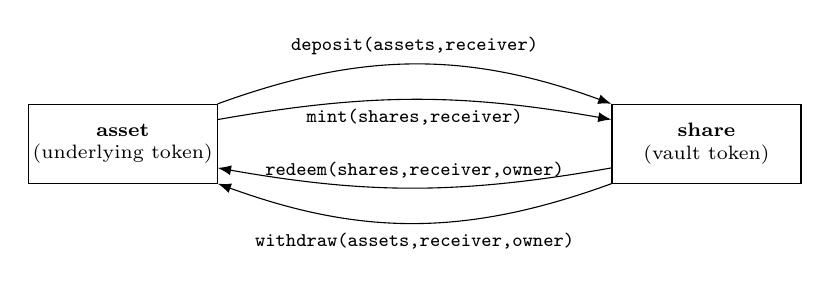
\begin{tikzpicture}[
  node distance=5cm,
  box/.style={minimum width=2.4cm, minimum height=1cm, inner sep=0pt, draw},
  >={Latex}
]

  \node[box] (A) {\shortstack{\scriptsize \textbf{asset} \\ \scriptsize (underlying token)}};
  \node[box, right=of A] (B) {\shortstack{\scriptsize \textbf{share} \\ \scriptsize (vault token)}};

  \draw[->] (A.north east) to[out=20,in=160]
    node[above, pos=0.5] {\scriptsize\texttt{deposit(assets,receiver)}} (B.north west);
  \draw[->] ([yshift=-0.2cm]A.north east) to[out=10,in=170]
    node[below, pos=0.5] {\scriptsize\texttt{mint(shares,receiver)}} ([yshift=-0.2cm]B.north west);

  \draw[<-] (A.south east) to[out=-20,in=-160]
    node[below, pos=0.5] {\scriptsize\texttt{withdraw(assets,receiver,owner)}} (B.south west);
  \draw[<-] ([yshift=0.2cm]A.south east) to[out=-10,in=-170]
    node[above, pos=0.5] {\scriptsize\texttt{redeem(shares,receiver,owner)}} ([yshift=0.2cm]B.south west);

\end{tikzpicture}

\end{frame}

\begin{frame}[fragile]{rebase token}

\begin{itemize}
  \item Rebase tokens change token quantity, while EIP-4626 tokens change token value.
  \item Don’t use share tokens. Balances are calculated by $balance = base\_balance \times ratio$ \\ On mint: $base\_balance = balance / ratio$
  \item The operator periodically adjusts the ratio to reflect value changes (e.g., staking rewards).
  \item Because balances change continuously, rebase tokens are hard to use in DeFi.
  %\item Rebase tokens can be wrapped into wrapped rebase tokens with the current balance.
\item Can wrap rebase tokens into EIP-4626-style shares \\ (e.g., stETH $\rightarrow$ wstETH, wrapped stETH).

\end{itemize}

\centering
\scalebox{0.8}{%
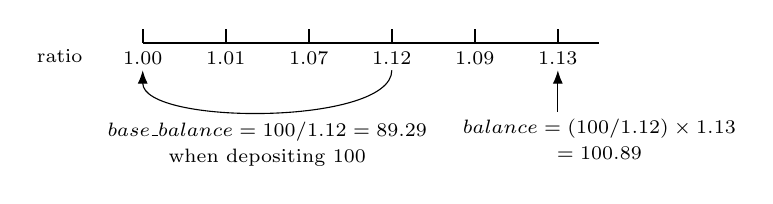
\begin{tikzpicture}[
    tick/.style={draw, thick},
    >={Latex}
]

\def\ticknums{1.00, 1.01, 1.07, 1.12, 1.09, 1.13}
\def\tickgap{3em}
\def\tickheight{0.5em}

\foreach \i [count=\n from 0] in \ticknums {
  \draw[tick] (\n*\tickgap,0) -- (\n*\tickgap,{\tickheight});
  \node[below] at (\n*\tickgap,0) {\scriptsize\i};
}
\draw[tick] (0,0) -- ({(\tickgap)*5.5},0);
\node at (-\tickgap,-\tickheight) {\scriptsize ratio};

\draw[->] (3*\tickgap,-2*\tickheight) .. controls +(0,-2em) and +(0,-2em) .. (0*\tickgap,-2*\tickheight) node[midway, below] {\shortstack{\scriptsize $base\_balance = 100 / 1.12 = 89.29$ \\ \scriptsize when depositing 100}};
\draw[->] (5*\tickgap,-5*\tickheight) -- (5*\tickgap,-2*\tickheight);
\node at (5.5*\tickgap,-7*\tickheight) {\shortstack{\scriptsize $balance = (100 / 1.12) \times 1.13$ \\ \scriptsize $= 100.89$}};

\end{tikzpicture}%
}

\end{frame}

\begin{frame}[fragile]{Fireblocks ERC20F}

\begin{itemize}
  \item \href{https://github.com/fireblocks/fireblocks-smart-contracts}{\faGithub\ fireblocks/fireblocks-smart-contracts}
  \item \texttt{grant/revokeRole()} and fine-grained roles like \texttt{UPGRADER\_ROLE}, \texttt{BURNER\_ROLE} and \texttt{SALVAGE\_ROLE}
  \item Both sender and recipient must be in the allowlist.
  \item ERC-2612 Permit and safer \texttt{increase/descreaseAllowance(spender,value)}
  \item \texttt{recoverTokens(address,amount)} revokes tokens from unlisted addresses
  \item rescue ERC-20 (\texttt{salvageERC20()}) or ETH (\texttt{salvageGas()}) accidentally sent to the token contract
  \item \texttt{mint/burn()}, \texttt{pause/unpause()}
  \item ERC-2771 meta transaction friendly gasless version, ERC20FGasless
  \item Example: WUSD (Worldwide USD), FRNT (Wyoming's Frontier)
\end{itemize}

\end{frame}

\begin{frame}[fragile]{privacy}

Economic privacy is important for B2B contracts, salaries, spending details, and so on. Unlike cash or e-cash, blockchains are inherently transparent. Privacy solutions have been proposed using techniques such as encryption, ZKP, and FHE.

\begin{description}
  \item[encryption] J.P. Morgan’s Quorum blockchain separates public state from privacy state and provides privacy transactions.
  \item[ZKP] Zerocash (the basis of Zcash and Tornado Cash) hides the sender, recipient, and amount by building a shielded pool. Various zkERC20 proposals, ERC-1724 Confidential Token, and EY Nightfall L2 fall into this category. Since Zerocash's UTXO model is unsuitable for DeFi, there have also been attempts to hide the account state in the account-based model, such as Zether.
  \item[FHE] Several solutions have emerged leveraging Zama’s FHE smart contract library.
\end{description}

\end{frame}

\begin{frame}[fragile]{*Passport}

\begin{itemize}
  \item ZKPassport and Self (OpenPassport, by Celo Marek)
  \item NFC reader extracts e-passport data and signature, that are encrypted with MRZ info to prevent unauthorized reading.
  \item[] \includegraphics[width=0.4\textwidth]{mrz}
  \item Present ZKP proving age, nationality, and issuing country conditions.
  \begin{itemize}
    \item age $\ge$ 18
    \item nationality not in SANCTIONED\_COUNTRIES
  \end{itemize}
  \item Limitations: \sout{forged signatures}, identity cloning, passport possession rate, passport revocation
\end{itemize}

%\includegraphics[height=3.0ex]{dsrv_logo_master_black}

\end{frame}

\begin{frame}[fragile]{Our token checklist}

% chain-level - DA
% https://github.com/ndaxio/ERC1400 consensys - t-rex와 유사 (certificate로 validate되야 transfer, force transfer)
% 8 billion people state

\begin{itemize}
  \item mint/burn, allowlist/denylist, freeze
  \item refund, escrow
  \item AA-friendly (gas sponsorship)
  \item KYC, AML, compliance, proof of reserve, trade record
  \item upgradeable contract with storage slot (EIP-1967)
  \item address and QR code generation
  \item social login and recovery
  \item on/off-ramp, oracle services
  \item monitoring, emergency action, pause, rescue
\end{itemize}

\begin{itemize}
  \item ERC-3643 needs pre-arranged identity info. How about on-demand indentity? Also, overhead of one contract per identity.
  \item scalability: ERC-7291 \texttt{Blacklist(\ldots,addresses,\ldots)} event with 8 billion people?
  \item scalability: $\num{22100}\,\text{gas}\,(32\,\text{bytes}) \times 8b \times 1\,\text{gwei/gas} = \text{\$}707m$ at \$4000/ETH $\longrightarrow$ accumulator-based, interface with proof input
\end{itemize}

\end{frame}

\end{document}
